\documentclass[a4paper, 11pt]{article}
\usepackage{lipsum} %This package just generates Lorem Ipsum filler text. 
\usepackage{fullpage} % changes the margin
\usepackage{mathpazo}
\usepackage{graphicx}
\usepackage{enumerate}
\usepackage{CJK}
\usepackage{amsmath,amsfonts,amsthm} % Math packages
\usepackage{listings}

\begin{document}
%Header-Make sure you update this information!!!!
\noindent
\large\textbf{Homework 1} \hfill \textbf{Hongyu Yan (516030910595)} \\
\normalsize {\bf CS 259 Numerical Methods for Data Science} \hfill ACM Class, Zhiyuan College, SJTU\\
Prof.~{\bf David Bindel} \hfill Due Date: Month Day, Year\\
TA.~{\bf Yurong You, Xinran Zhu} \hfill Submit Date: \today

\section*{Problem 1}
The plot is shown in figure 1:

\begin{figure}[ht]
\centering
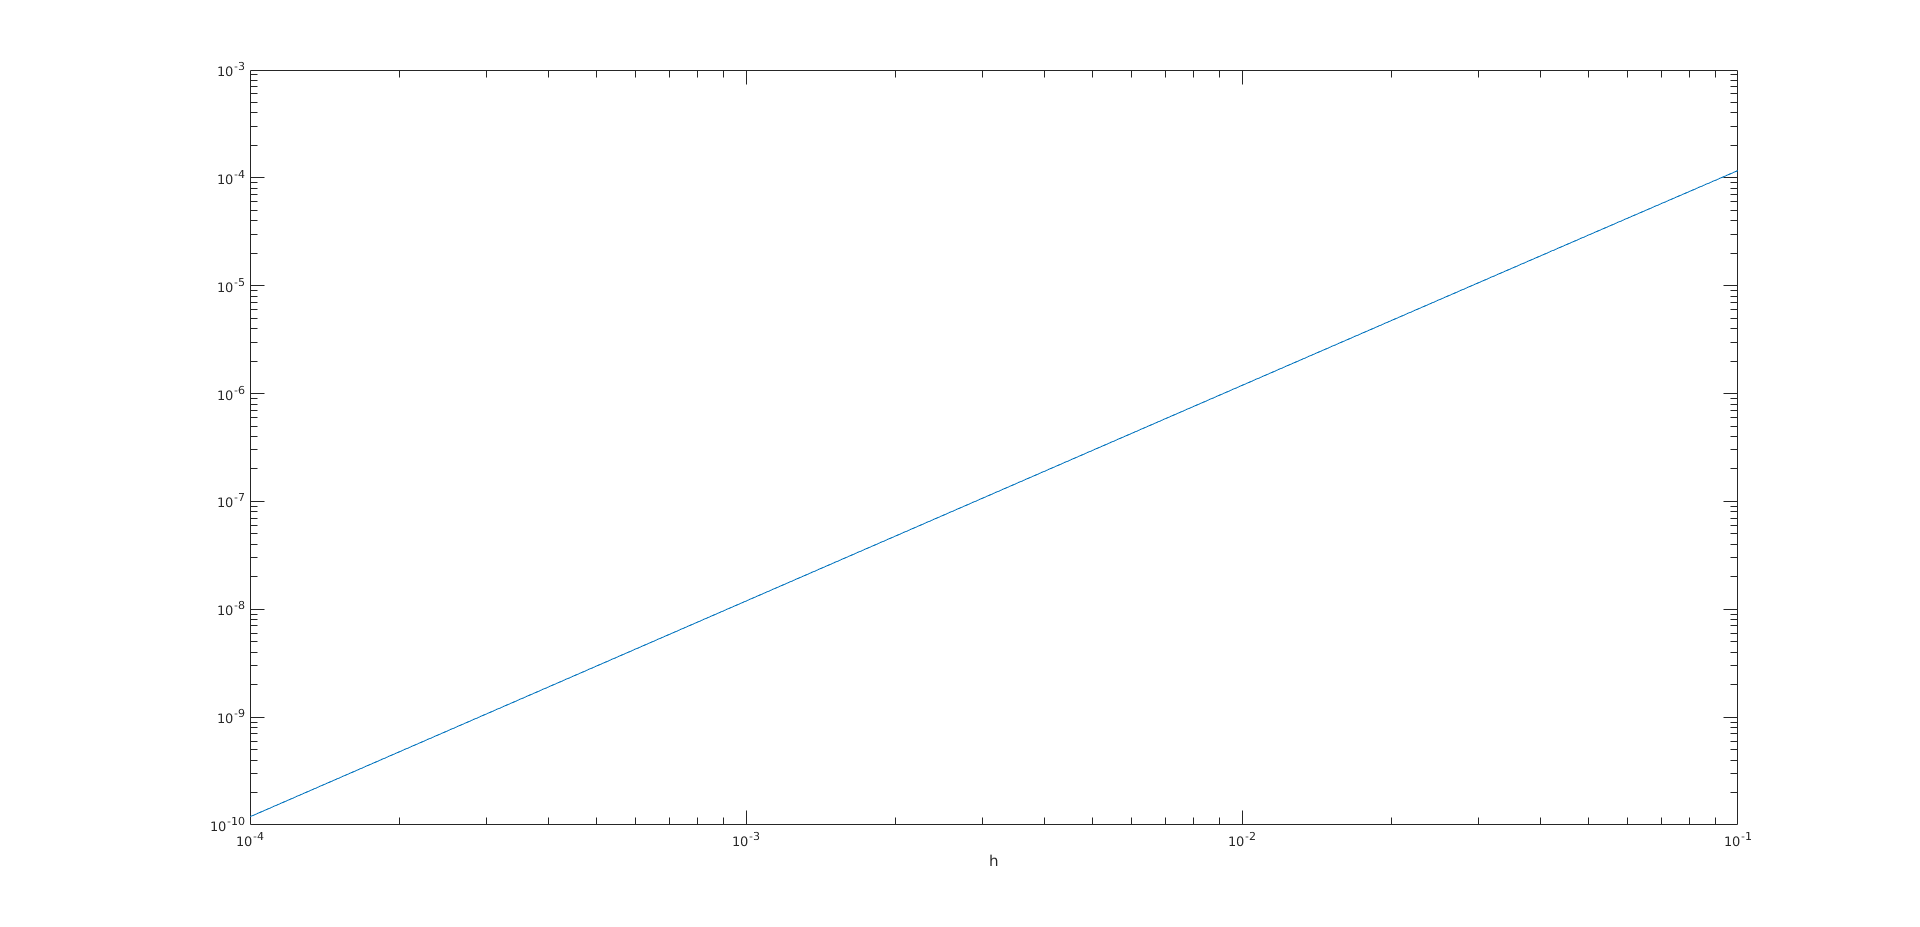
\includegraphics[scale=0.3]{figure/problem1.png}
\caption{the log-log plot of the norm versus h}
\label{fig1}
\end{figure}

The result of fitting the curve with MATLAB Curve Fitting Tool is as below.
\begin{figure}[ht]
\centering
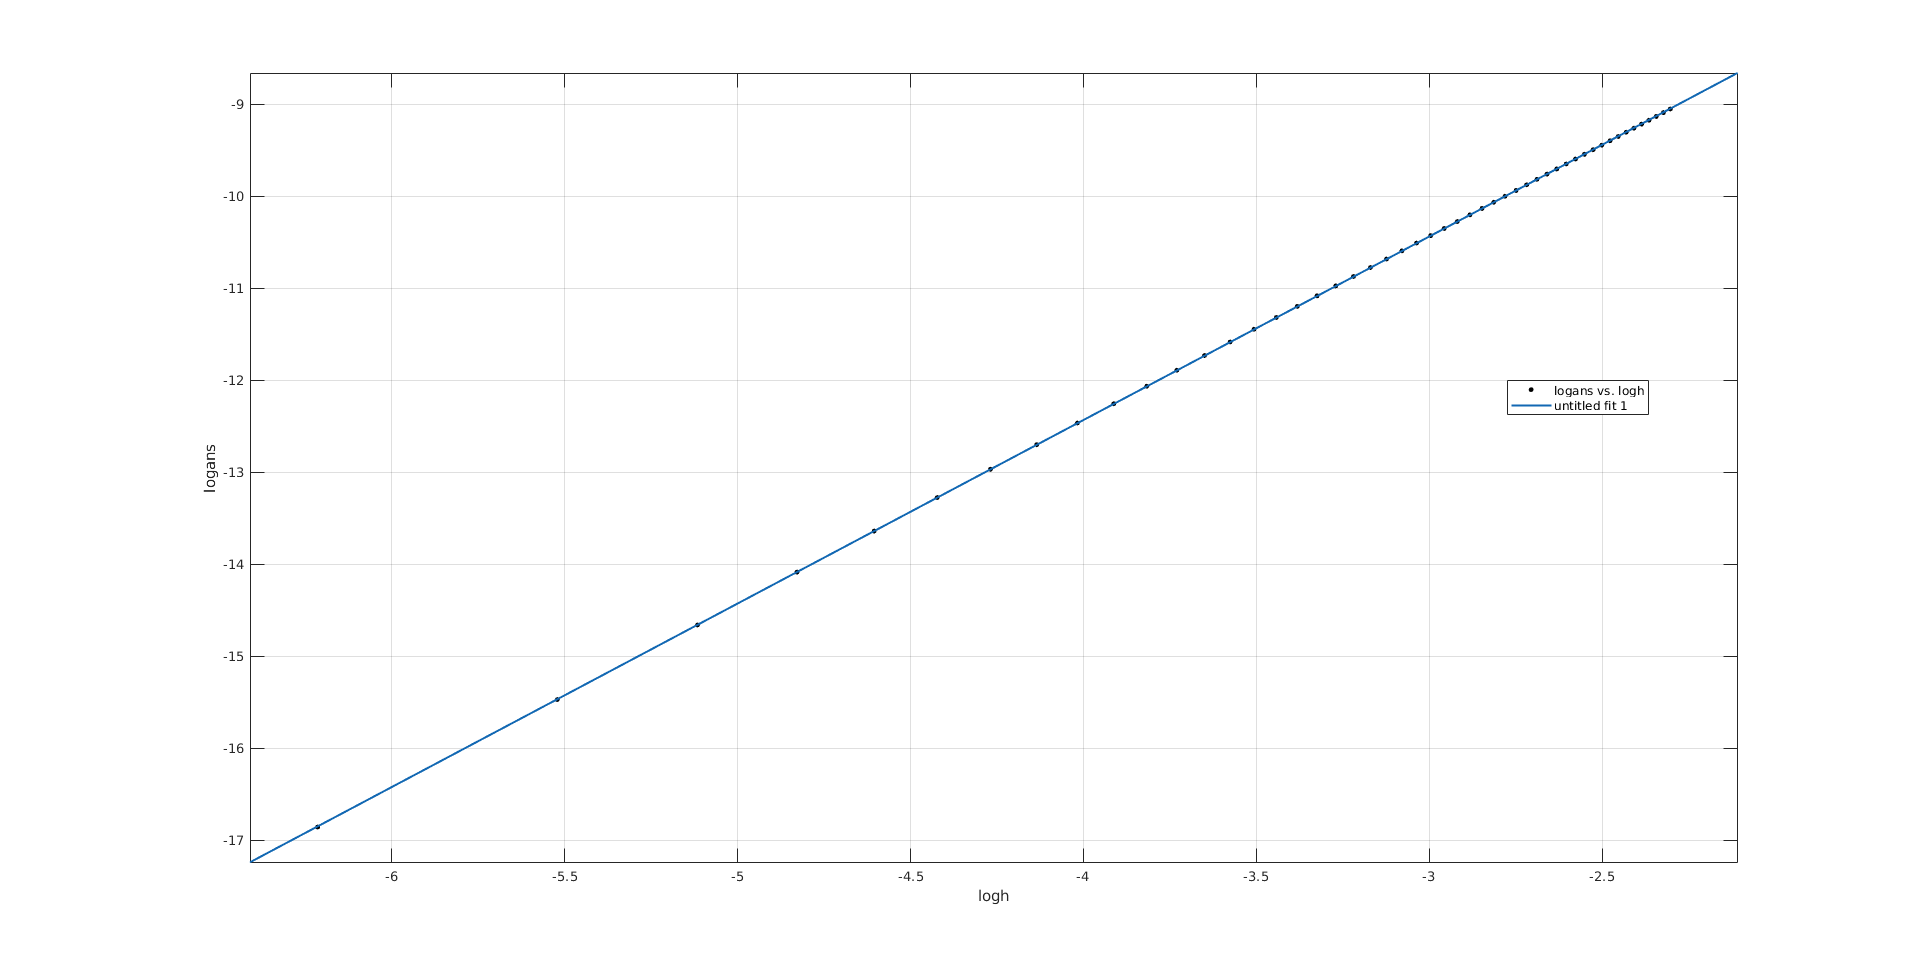
\includegraphics[scale=0.3]{figure/problem1_fit.png}
\caption{the fitting curve of log(h) versus log(norm)}
\label{fig2}
\end{figure}
\lstset{
	language=bash,
	xleftmargin=3em,
}
\begin{lstlisting}
Linear model Poly1:
     f(x) = p1*x + p2
Coefficients (with 95% confidence bounds):
       p1 =       1.994  (1.993, 1.995)
       p2 =      -4.458  (-4.461, -4.456)

Goodness of fit:
  SSE: 0.0002814
  R-square: 1
  Adjusted R-square: 1
  RMSE: 0.002421
\end{lstlisting}

\par
\subsection*{Proof}

\begin{align*}
	  & (A+hE)^{-1}-(A^{-1}-hA^{-1}EA^{-1})  \\
	= & (A+hE)^{-1}[I-(A+hE)(I-hA^{-1}E)]A^{-1} \\
	= & (A+hE)^{-1}[I-A(I+hA^{-1}E)(I-hA^{-1}E)]A^{-1} \\
	= & (A+hE)^{-1}[I-I-Ah^2(A^{-1}E)^2A^{-1}] \\
	= & h^2(A+hE)^{-1}A(A^{-1}E)^2A^{-1}
\end{align*}

Since h is small, we have $A+hE \approx A$. Then the result approximates $||h^2(A^{-1}E)^2A^{-1}||=||h^2|| *||(A^{-1}E)^2A^{-1}||$, so $\frac{log(result)}{log(h)}=2$ , which means the asymptotic slope on the log-log plot is 2.

\section*{Problem 2}
\subsection*{The KKT conditions}
The lagrangian is
$$
L(x, \lambda, \mu) = ||x-u||^2 + \lambda\sum_i x_i+ \sum_i \mu_i(-x_i)
$$

So the KKT conditions are:

\begin{align*}
  2x-2u+\lambda e-\mu &= 0 \\
  \sum_i x_i - 1      &= 0,     & \mbox{equality constraints}\\
  -x_i                & \leq 0, & \mbox{inequality constraints}\\
  \mu_i               & \geq 0, & \mbox{non-negativity of multipliers}\\
  -x_i \mu_i          &= 0,     & \mbox{complementary slackness}
\end{align*}

e is $[1, 1, \cdots , 1]^T$, $\mu$ is $[\mu_1, \mu_2, \cdots, \mu_n]^T$
\subsection*{Proof}
From the KKT conditions we have:
\begin{align*}
	2x-2u+\lambda e-\mu & = 0 \\
	                 x & = u - \frac{\lambda e-\mu}{2} \\
	               x_i & = u_i - \frac{\lambda - \mu_i}{2}
\end{align*}

So in some conditions, solution satisfies $x_i = max(u_i + C, 0)$.

In such condition, $C=\frac{\lambda}{2}$, according to $-x_i\mu_i = 0$, we have:
\begin{align*}
 x_i=0, u_i-\frac{\lambda}{2} < 0 &, &when\ \mu_i > 0 \\
  x_i = u_i-\frac{\lambda}{2}&, &when\ \mu_i = 0 
\end{align*}


\end{document}
